An electric vehicle charging station, also called EV charging station is an element in an infrastructure that supplies electric energy for the recharging of electric vehicles, such as plug-in electric vehicles and plug-in hybrids. At home or work, some electric vehicles have onboard converters that can plug into a standard electrical outlet or a high-capacity appliance outlet. 

However, in most cases, others require a charging station that provides electrical conversion, monitoring, or safety functionality. These stations are also needed when travelling, and many support faster charging at higher voltages and currents that are available from residential EVSEs. Public charging stations are typically on-street facilities provided by electric utility companies or located at retail shopping centers and operated by many private companies.

Nowadays, electric vehicles become more and more popular as people want to cut down the pollution and cost of the usage of traditional energy. When most people considering whether to switch to an electric car, the most worrying aspect is the development of charging stations, which directly impact the usability of the electric car.

EVs in China is experiencing an overall growth in the past few years, which directly results in the massive construction and modification of charging stations and current road networks. Fig.\ref{fig1} shows the global distribution of an operators' charging stations in Shanghai, where there are over 600 stations. However, the cost of construction of charging stations is considerable and are often very costly or even impracticable to reallocate. This raise the question of how to select the locations for building the charging stations. In a typical view, a charging station no matter where it is located, its 'success' is often determined by the use rate of a station.

\begin{figure}[!htp]
	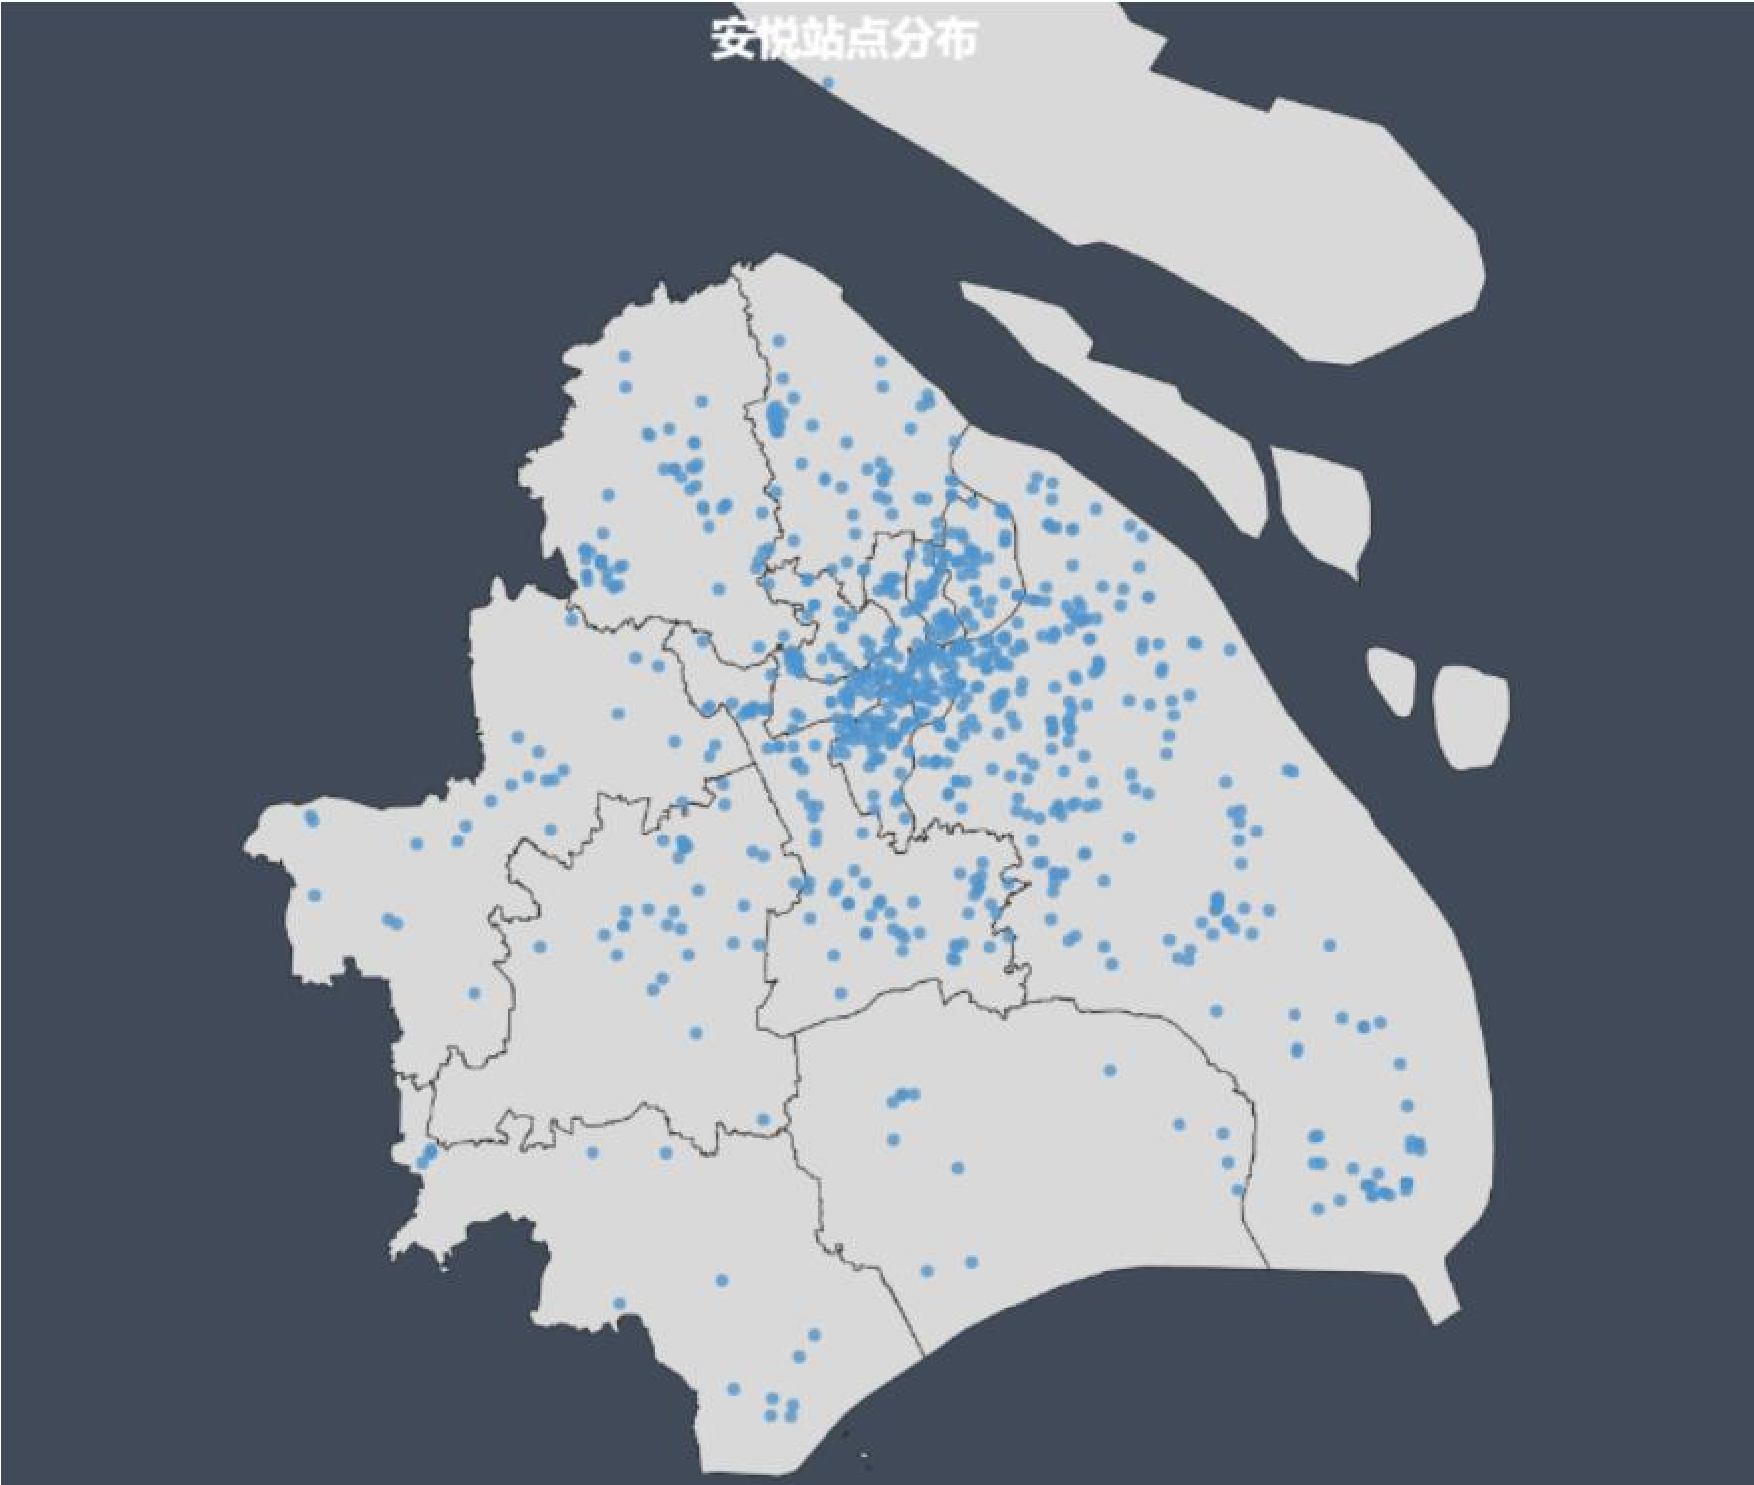
\includegraphics[width=\columnwidth]{./figures/areas.pdf}
	\centering
	\caption{Distribution of charing stations in Shanghai, China}
	\label{fig1}
\end{figure}  

In order to help with station setting strategies, we explore a time frame based prediction framework to classify stations into high use rate and low use rate in various time frames, using features like georaphical information as well as other working elements. We set 8 time frames in total, they are total time, weekdays, weekends, mornings, evenings, moring\_rush hours, evening\_rush hours and travel hours. As for features, we choose longitude, latitude, Point of Interests(POIs), charging price, AC/DC charging types and whether it's private or public to use.

We make use of an operator's charging station data in Shanghai and  have kept collecting the use rate value for about a month, then we seperate the whole use rate dataset into various time frames that we have already planned. At the same time, we also collect important featrure data as formerly said. Both of the two datasets require a data cleaning procedure, in order to filter some invalid data or outliers. Furthermore, we make some analyses on features that we confirm to have significant impact on station's use rate.

We evaluate our method with four machine learning algorithm, they are RL, Random Forest, SVM and XGBOOST respectively. In each time frame, with features put into it, the model will tell which level of use rate that a station belongs to. Experimental results show that geopraphical information as well as working elements of a station do have great influence on its use rate, which can bring operators some enlightment on location choosing for station construction.

In summary, the contributions of this work are listed as follows:
\begin{itemize}
	\item We propose a time frame based prediction framework to classify whether a staion is of high use rate or low use rate based on operator's charging station data and important features.
	\item We make detailed analyses on both of the two datasets to obtain basic information and find the relationships between station's use rate and those features.
	\item We make use of four learning models for improving the accuracy of use rate prediction and achieve relatively favorable results.
\end{itemize}

The rest of this paper is organized as follows: Section 2 gives definition of the problem. Section 3 reviews some related work done before. Section 4 describes work on collected dataset and feature analyses. Section 5 provides experiments with four machine learning algorithms and the results. In Section 6, we draw a conclusion to the paper and make discussions on future work.
